\documentclass[a4paper,11pt,stu]{apa}

% Turn off page number
\thispagestyle{empty}

% Rotate page to landscape
\usepackage[landscape]{geometry}

% Set double spacing
\usepackage{setspace}

% Set captions
\usepackage[
    format=plain,
    font={up,normalsize},
    labelfont={it,bf},
    textfont=it,
    labelsep=newline]{caption}
\captionsetup{
    justification=raggedright,
    singlelinecheck=false,
    margin=0cm
    } % Align left
%\AtEveryCite{\normalfont} % Prevent italic anywhere else in the document
\usepackage[capposition=top]{floatrow} % For ``Note.'' underneath the figures
%\DeclareCaptionFont{normal}{\fontsize{11}{13.2}\selectfont}
%\newcommand{\fignote}[1]{\floatsetup{font=normal,cappositon=bottom}\floatfoot{\large \textit{Note.} #1}}

\usepackage{tikz}
\usetikzlibrary{automata,shapes,arrows,calc,positioning,decorations.pathmorphing}

\begin{document}

\begin{figure}[!h]
\caption{Latent Growth Curve Models for MST Effectiveness}
\label{fig:mst}

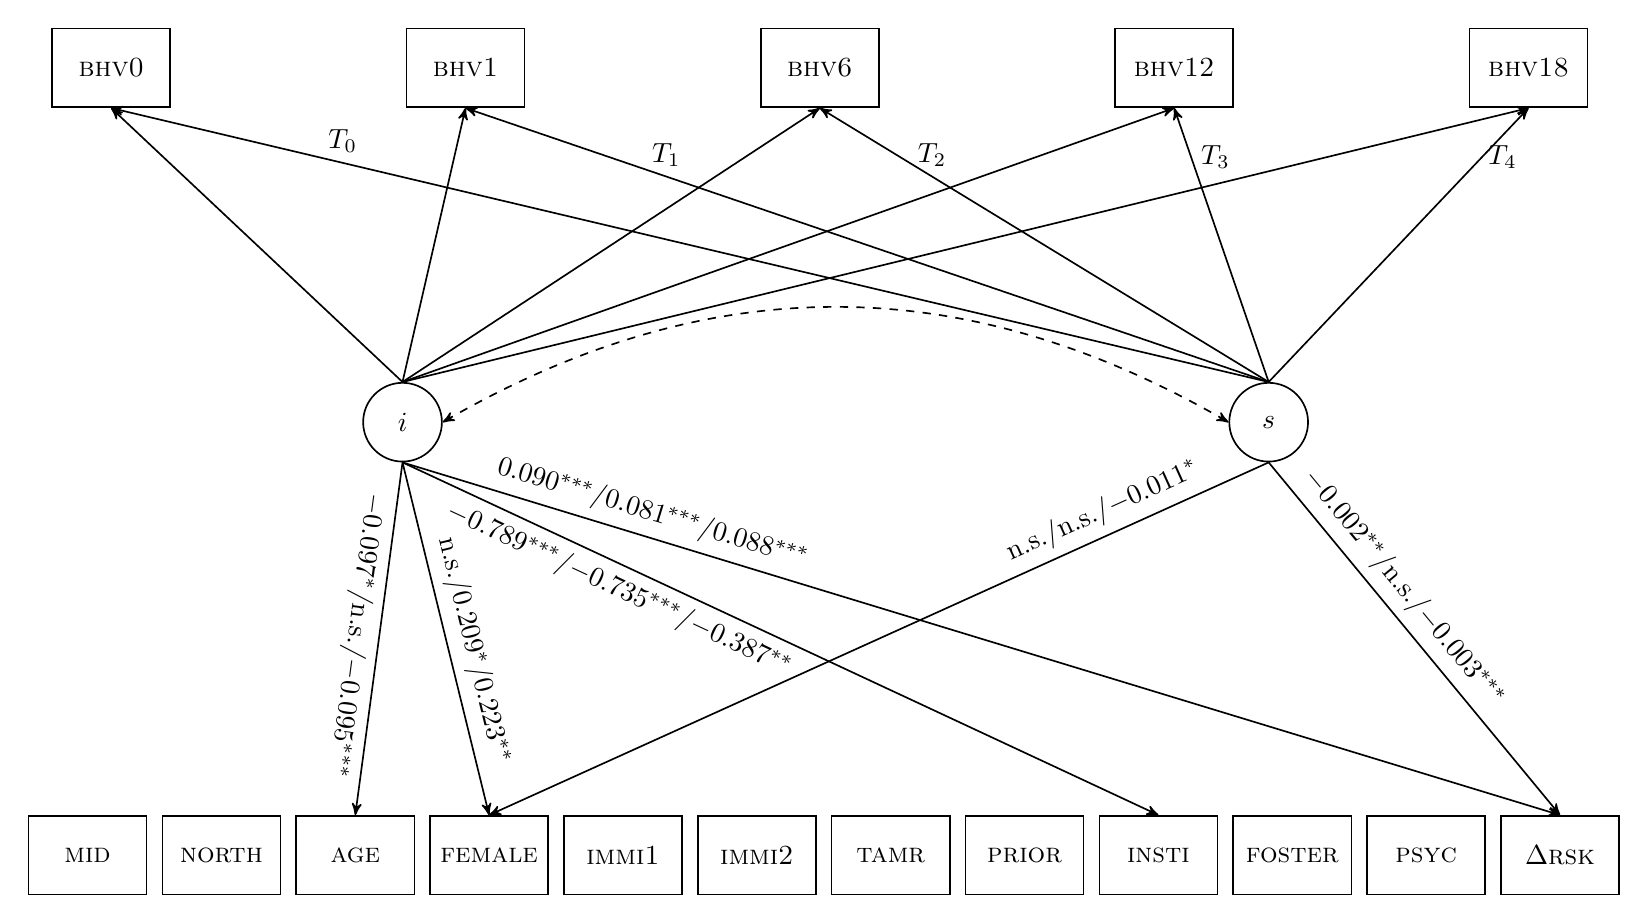
\begin{tikzpicture}[
    latvar/.style={ellipse,draw=black,minimum width=1cm,minimum height=1cm},
    manvar/.style={rectangle,draw=black,minimum width=1.5cm,minimum height=1cm},
    misvar/.style={dashed,rectangle,draw=black,minimum width=1cm,minimum height=1cm},
    mean/.style={fill=black!10!white,regular polygon,regular polygon sides=3},
    ->,>=stealth',semithick,
    bend angle=30,
    decoration={
        zigzag,
        amplitude=1pt,
        segment length=1mm,
        post=lineto,
        post length=4pt
    }
]

% Draw covariates
% R> seq(0, 20, 1.7)
\node[manvar] (x1) at (0,0) {\textsc{mid}};
\node[manvar] (x2) at (1.7,0) {\textsc{north}};
\node[manvar] (x3) at (3.4,0) {\textsc{age}};
\node[manvar] (x4) at (5.1,0) {\textsc{female}};
\node[manvar] (x5) at (6.8,0) {\textsc{immi1}};
\node[manvar] (x6) at (8.5,0) {\textsc{immi2}};
\node[manvar] (x7) at (10.2,0) {\textsc{tamr}};
\node[manvar] (x8) at (11.9,0) {\textsc{prior}};
\node[manvar] (x9) at (13.6,0) {\textsc{insti}};
\node[manvar] (x10) at (15.3,0) {\textsc{foster}};
\node[manvar] (x11) at (17,0) {\textsc{psyc}};
\node[manvar] (x12) at (18.7,0) {$\Delta$\textsc{rsk}};

% Draw i and s
\node[latvar] (i) at (4,5.5) {$i$};
\node[latvar] (s) at (15,5.5) {$s$};

% Draw outcome variables
% R> seq(0.3, 19, 4.5)
\node[manvar] (y0) at (0.3,10) {\textsc{bhv0}};
\node[manvar] (y1) at (4.8,10) {\textsc{bhv1}};
\node[manvar] (y2) at (9.3,10) {\textsc{bhv6}};
\node[manvar] (y3) at (13.8,10) {\textsc{bhv12}};
\node[manvar] (y4) at (18.3,10) {\textsc{bhv18}};

% Link i to y
\draw[->] (i.north) to (y0.south);
\draw[->] (i.north) to (y1.south);
\draw[->] (i.north) to (y2.south);
\draw[->] (i.north) to (y3.south);
\draw[->] (i.north) to (y4.south);

% Link s to y
\draw[->] (s.north) to node[above,pos=0.8] {$T_0$} (y0.south);
\draw[->] (s.north) to node[above,pos=0.75] {$T_1$} (y1.south);
\draw[->] (s.north) to node[above,pos=0.75] {$T_2$} (y2.south);
\draw[->] (s.north) to node[right,pos=0.82] {$T_3$} (y3.south);
\draw[->] (s.north) to node[below,pos=0.9] {$T_4$} (y4.south);

% Allow correlation between i and s
\draw[dashed,<->] (i.east) to [bend left] (s.west);

% Link x to i
% age
\draw[<-] (x3.north) to node[below,sloped,rotate=180] {$-0.097^{*}$/n.s./$-0.095^{***}$} (i.south);
% female
\draw[<-] (x4.north) to node[above,sloped,pos=0.45] {n.s./$0.209^{*}$/$0.223^{**}$} (i.south);
% insti
\draw[<-] (x9.north) to node[below,sloped,pos=0.7] {$-0.789^{***}$/$-0.735^{***}$/$-0.387^{**}$} (i.south);
% chgyls
\draw[<-] (x12.north) to node[above,sloped,pos=0.79] {$0.090^{***}$/$0.081^{***}$/$0.088^{***}$} (i.south);

% Link x to s
% female
\draw[<-] (x4.north) to node[above,sloped,pos=0.8] {n.s./n.s./$-0.011^{*}$} (s.south);
% chgyls
\draw[<-] (x12.north) to node[above,sloped,pos=0.6] {$-0.002^{**}$/n.s./$-0.003^{***}$} (s.south);

\end{tikzpicture}

\floatfoot{\normalsize \textit{Note.} These latent growth curve models evaluate variables associated with MST effectiveness across the COVID-19 pandemic. The intercept ($i$) carries factor loadings of $1$s (omitted) to all outcome variables while the slope ($s$) carries time stamps measured in months as factor loadings from $T_0$ to $T_4$. Intervals between admission ($T_0$) and discharge ($T_1$) vary by clients. All subsequent time points are six months apart, representing 6-, 12-, and 18-months follow-up measures. The dashed arrow suggests no significant covariations between intercepts and slopes, hence growth curves do not fan in or out. Unstandardised coefficients are reported in the order \textsc{before}/\textsc{during}/\textsc{after} COVID-19 lockdowns at MST admissions. Covariates receiving no arrows provide insufficient explanatory power for growth curves.

n.s. = not significant at $\alpha=.05$ level, $^{*}p<.05$, $^{**}p<.01$, $^{***}p<.001$.}

\end{figure}

\end{document}